\documentclass[12pt]{article}
\usepackage{graphicx}
\usepackage{float}
\usepackage{url}
\usepackage{hyperref}
\usepackage{subcaption}
\usepackage{amsmath}
\usepackage[style=numeric,sorting=none,maxbibnames=9,autopunct=true,babel=hyphen,hyperref=true,backend=biber]{biblatex}

\bibliography{references}
\graphicspath{{./Graphs/}}
\begin{document}

\title{Cosmology with Galaxy Clusters \\ Cosmology Project}
\author{Carlos Rafael Salazar Letona \\ s21205751}
\maketitle

\section{Introduction}
In this project, different cosmological quantities were studied. First, the cosmological distances, as well as the differential volume are calculated from the rescaled Hubble parameter data for different cosmologies. Then, from the maximum observable flux of the XXL survey\cite{ref:xxlsurvey}, the maximum redshift at which objects can be detected is calculated, as well as the observable mass range. As a third task, using the power spectrum, the mass variance and non-linear mass scales are determined. Lastly, the number of expected haloes for a region of the sky that can be observed is calculated.

The quantities in this project were calculated for different cosmologies, however, here only the results for the $\Lambda$CDM model will be presented, as it is the standard model of cosmology.

\subsection{$\Lambda$CDM model}
The $\Lambda$CDM model is considered the standard model of cosmology, as it is the simplest theory that reproduces the most important results, such as \cite{ref:lambdacdm}:

\begin{enumerate}
\item the existence and structure of the CMB
\item the large-scale structure in the distribution of galaxies
\item the observed abundances of the lightest atoms
\item the accelerating expansion of the universe
\end{enumerate}
In this model, the energy of the universe is divided in three components: dark energy, cold dark matter, and ordinary matter.


\subsection{Power Spectrum}
The power spectrum is used to describe the density contrast of the universe, and it is calculated using the Fourier transform of the matter correlation function\cite{ref:powerspectrum}.


\section{Cosmological distances}
The following cosmological distances were calculated using the rescaled Hubble parameter. They can be seen together in fig~\ref{fig:cosmoDistances}.

\subsection{Comoving radial distance}
\begin{equation}
	\chi(z) = \int_{0}^{z}\frac{cdz}{H(z)} = \frac{c}{H_{0}} \int_{0}^{z}\frac{dz}{E(z)}
	\label{eq:comovingDist}
\end{equation}

\subsection{Luminosity distance}
\begin{equation}
	d_{L}(z) = (1 + z)  \chi(z)
	\label{eq:lumDist}
\end{equation}

\subsection{Angular distance}
\begin{equation}
	d_{A}(z) = \frac{\chi(z)}{1 + z}  
	\label{eq:angDist}
\end{equation}

\subsection{Diameter distance}
In the case of the $\Lambda$CDM model, the diameter distance will be equal to the comoving radial distance, as it is the model for flat space (k = 0).
\begin{equation}
	d_{k} = S_{k}(\chi(z))
	\label{eq:diamDist}
\end{equation}
\begin{equation}
	S_{k}(x) = \begin{cases}
		\sin(x), & \text{if $k = 1$}\\
		x, & \text{if $k = 0$}\\
		\sinh(x), & \text{if $k = -1$}
	  \end{cases}
	\label{eq:diamDist2}
\end{equation}

\begin{figure}[h]
	\centering
	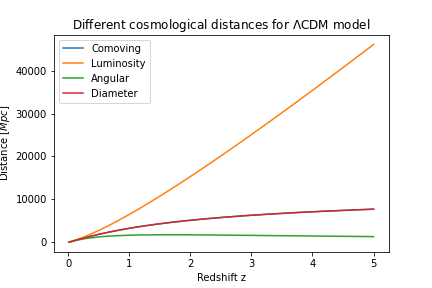
\includegraphics[width=0.6\linewidth]{cosmoDistances.png}
	\caption{Different cosmological distances for the $\Lambda$CDM model of cosmology.}
	\label{fig:cosmoDistances}
\end{figure}

\subsection{Volume}
Then, from the diameter distance, the volume could be calculated. More specifically, the differential volume of a square region of sky, with an area given by the angle $\Omega^{2}$, and at redshift z. This is given by:
\begin{equation}
	\frac{dV}{dz} = \Omega^{2} \left( \frac{c}{H_{0}} \right)^{3} \frac{d_{k}(z)^{2}}{E(z)}
	\label{eq:diffVolume}
\end{equation}
After integration, the volume of a section of sky, starting from redshift 0, and going to redshift 5 (in this case) is obtained. The relationship between volume and redshift can be seen in fig~\ref{fig:volLCDM}.

\begin{figure}[ht]
	\centering
	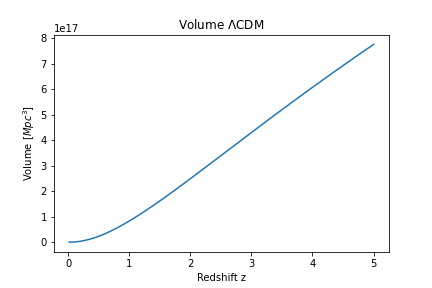
\includegraphics[width=0.6\linewidth]{volumeLCDM.png}
	\caption{Volume as a function of redshift.}
	\label{fig:volLCDM}
\end{figure}

It can also be interesting to see how the volume changes when choosing different starting and ending redshifts. This can be seen on the contour on fig~\ref{fig:volContour}. It can be noted that, as expected, the volume is the highest for small initial redshift and large final redshift, as they represent a larger portion of space.

\begin{figure}[ht]
	\centering
	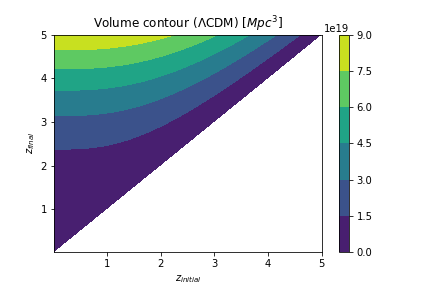
\includegraphics[width=0.6\linewidth]{volContour.png}
	\caption{Volumes for different initial and final redshifts.}
	\label{fig:volContour}
\end{figure}



\section{Flux and observable range of XXL survey}
The flux can be calculated from the luminosity, and the luminosity distance. Given by equation:
\begin{equation}
	F = \frac{L}{4 \pi d_{L}^{2}}
	\label{eq:flux}
\end{equation}
Where the luminosity distance is a function of the redshift, therefore for a fixed luminosity value $L$, we get a flux as a function of the redshift. In the XXL survey, there is a limiting flux, under which no more objects can be observed. The limiting flux, $f_{lim}$ is equal to $1.3 \cdot 10^{-14}$~\cite{ref:xxlsurvey}. The redshift value at which the graph intersects the limiting flux will give us the maximum redshift at which an object with luminosity $L$ will be visible. This process can be done for the different $L$ values (as shown in fig~\ref{fig:fluxZmax}), in order to find a relation between maximum redshift and luminosity.

\begin{figure}[ht]
	\centering
	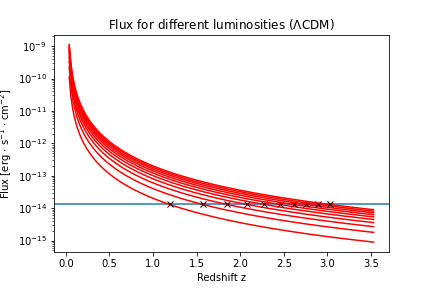
\includegraphics[width=0.6\linewidth]{fluxZmax.png}
	\caption{Flux as a function of redshift.}
	\label{fig:fluxZmax}
\end{figure}

The relation between maximum redshift and luminosity can be seen in fig~\ref{fig:zmax}. From this relation, the mass can also be calculated. From this, we obtain the mass that can be observed at certain redshifts.

\begin{equation}
	M_{500} = \left( \frac{L}{\left( \frac{h}{0.72} \right)^{-0.39} L^{*} E(z)^{\gamma}} \right)^{1/\alpha} M^{*}
	\label{eq:massLuminosity}
\end{equation}

\begin{figure}[ht]
	\centering
	\begin{subfigure}[b]{0.49\textwidth}
		\centering
		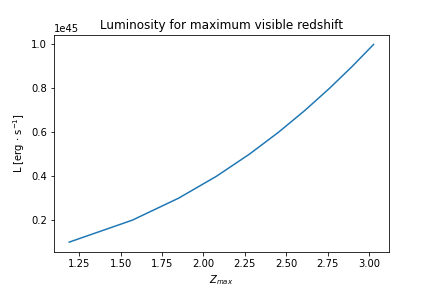
\includegraphics[width=\textwidth]{luminosityZmax.png}
	\end{subfigure}
	\hfill
	\begin{subfigure}[b]{0.49\textwidth}
		\centering
		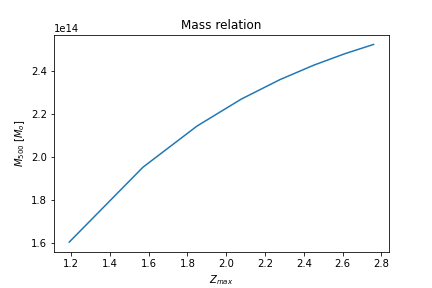
\includegraphics[width=\textwidth]{massZmax.png}
	\end{subfigure}
	\caption{Luminosity as a function of maximum redshift (left). Observable mass for different redshifts (right).}
	\label{fig:zmax}
\end{figure}



\section{Mass variance and non-linear mass scale}
The mass variance function is given by\cite{ref:halofunction}:
\begin{equation}
	\sigma^{2}(R) = \frac{D_{+}^{2}}{4 \pi^{2}} \int_{0}^{\infty} W^{2}(kR) P(k) k^{2} dk
	\label{eq:massVariation}
\end{equation}
Where, $W(k)$ is a window function used to select a given region. $P(k)$ is the power spectrum, $D_{+}$ is the growth factor, and $k$ is the wave number. The window function chosen for this project is:
\begin{equation}
	W(x) = \frac{3}{x^{3}} \left( \sin(x) - x \cos(x) \right)
	\label{eq:windowFunction}
\end{equation}

\begin{figure}[ht]
	\centering
	\begin{subfigure}[b]{0.49\textwidth}
		\centering
		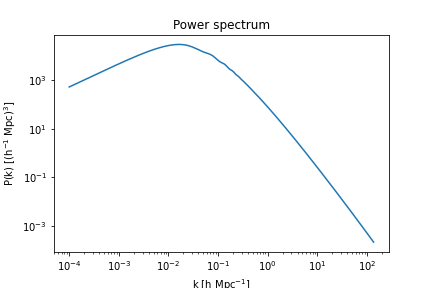
\includegraphics[width=\textwidth]{powerSpectrum.png}
	\end{subfigure}
	\hfill
	\begin{subfigure}[b]{0.49\textwidth}
		\centering
		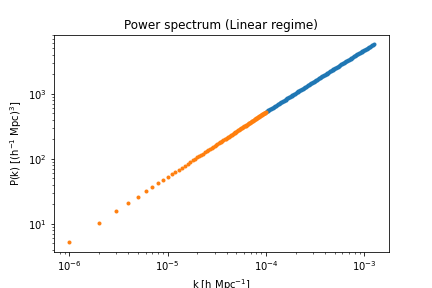
\includegraphics[width=\textwidth]{powerLinear.png}
	\end{subfigure}
	\begin{subfigure}[b]{0.49\textwidth}
		\centering
		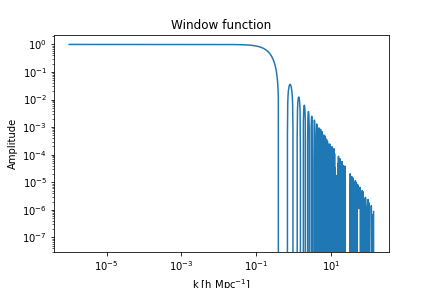
\includegraphics[width=\textwidth]{windowFunction.png}
	\end{subfigure}
	\caption{Power spectrum, the linear interpolation of the power spectrum on the liner regime, and the window function.}
	\label{fig:spectrums}
\end{figure}

The power spectrum was interpolated in the linear regime, in order to have a better data set for the integration. First, the value of $\sigma^{8}$ was calculated, such that the normalization constant could be calculated, which would ensure a value of $\sigma^{8} = 0.82$.

The mass variance is thus, a function of R. However, it also depends on the redshift, which for the previous case was set to 0. By plotting also the graphs for different redshifts, and finding the intercepts with the $x=1$ axis, the non-linear mass scale can be found (Following a procedure similar to the one used to find the maximum redshift for different luminosities in the previous subsection).

\begin{figure}[ht]
	\centering
	\begin{subfigure}[b]{0.49\textwidth}
		\centering
		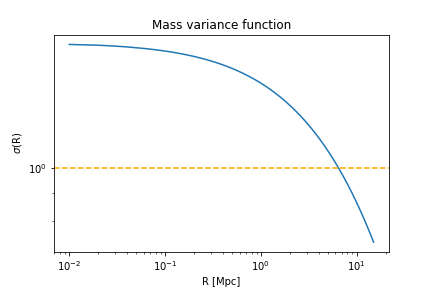
\includegraphics[width=\textwidth]{massVariance.png}
	\end{subfigure}
	\hfill
	\begin{subfigure}[b]{0.49\textwidth}
		\centering
		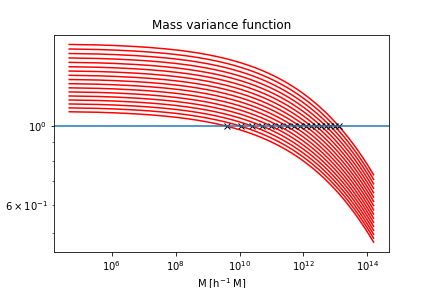
\includegraphics[width=\textwidth]{varianceMNL.png}
	\end{subfigure}
	\begin{subfigure}[b]{0.49\textwidth}
		\centering
		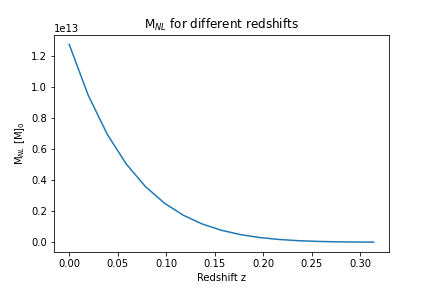
\includegraphics[width=\textwidth]{mnlRedshift.png}
	\end{subfigure}
	\caption{Mass variance as a function of $R$, mass variance of different redshifts and the intercepts with $x=1$, and the resulting $M_{NL}$ values as a function of redshift.}
	\label{fig:nonlinearScale}
\end{figure}



\section{Number counts of haloes}
The expected number of haloes for a given region of space was calculated using the Press-Schechter model. After having calculated the mass variance, it is possible to calculate the mass function $\Phi(M)$, defined as:
\begin{equation}
	\Phi(M) = \frac{dn}{dM} = \frac{\rho_{m}}{M^{2}} \frac{d \log \sigma^{-1}(M)}{d \log M} f(\nu)
	\label{eq:massFunction}
\end{equation}
where, $f(\sigma)$ is the multiplicity function, and $\nu = \delta / \sigma$ is the height. The Press-Schechter multiplicity function is\cite{ref:pressSchechter}:
\begin{equation}
	f(x) = \frac{x \sqrt{2}}{\sqrt{\pi}} e^{-\frac{x^{2}}{2}}
	\label{eq:multiplicityFunction}
\end{equation}

Then, the number of haloes can be calculated using the differential volume, and the integral of the mass function.
\begin{equation}
	N(>f_{min}) = \int_{z_{min}}^{z} \frac{dV}{dz} dz \int_{M_{min}}^{\infty} \Phi(M) dM
	\label{eq:haloCount}
\end{equation}

The minimum mass and redshift are obtained from the minimum value of the mass relation in fig~\ref{fig:zmax}. That is, the minimum masses that can be observed by the XXL survey. The result after calculating the two integrals is: $N(>f_{min}) = 173925.94$.


\section*{References}
\printbibliography[heading=none]

\end{document}